% ========================================
%	Header einbinden
% ========================================

\documentclass[bibtotoc,titlepage]{scrartcl}

% Deutsche Spracheinstellungen
\usepackage[ngerman,german]{babel, varioref}
\usepackage[T1]{fontenc}
\usepackage[utf8]{inputenc}

%\usepackage{marvosym}

\usepackage{amsfonts}
\usepackage{amssymb}
\usepackage{amsmath}
\usepackage{amscd}
\usepackage{amstext}
\usepackage{float}
\usepackage{caption}
\usepackage{wrapfig}
\usepackage{setspace}
\usepackage{threeparttable}
\usepackage{footnote}

\newfloat{formel}{htbp}{for}
\floatname{formel}{Formel}


\usepackage{longtable}

%\usepackage{bibgerm}

\usepackage{footnpag}

\usepackage{ifthen}                 %%% package for conditionals in TeX
\usepackage[amssymb]{SIunits}
%Fr textumflossene Bilder und Tablellen
%\usepackage{floatflt} - veraltet

%Fr Testzwecke aktivieren, zeigt labels und refs im Text an.
%\usepackage{showkeys}

% Abstand zwischen zwei Abs�zen nach DIN (1,5 Zeilen)
% \setlength{\parskip}{1.5ex plus0.5ex minus0.5ex}

% Einrckung am Anfang eines neuen Absatzes nach DIN (keine)
%\setlength{\parindent}{0pt}

% R�der definieren
% \setlength{\oddsidemargin}{0.3cm}
% \setlength{\textwidth}{15.6cm}

% bessere Bildunterschriften
%\usepackage[center]{caption2}


% Probleml�ungen beim Umgang mit Gleitumgebungen
\usepackage{float}

% Nummeriert bis zur Strukturstufe 3 (also <section>, <subsection> und <subsubsection>)
%\setcounter{secnumdepth}{3}

% Fhrt das Inhaltsverzeichnis bis zur Strukturstufe 3
%\setcounter{tocdepth}{3}

\usepackage{exscale}

\newenvironment{dsm} {\begin{displaymath}} {\end{displaymath}}
\newenvironment{vars} {\begin{center}\scriptsize} {\normalsize \end{center}}


\newcommand {\en} {\varepsilon_0}               % Epsilon-Null aus der Elektrodynamik
\newcommand {\lap} {\; \mathbf{\Delta}}         % Laplace-Operator
\newcommand {\R} { \mathbb{R} }                 % Menge der reellen Zahlen
\newcommand {\e} { \ \mathbf{e} }               % Eulersche Zahl
\renewcommand {\i} { \mathbf{i} }               % komplexe Zahl i
\newcommand {\N} { \mathbb{N} }                 % Menge der nat. Zahlen
\newcommand {\C} { \mathbb{C} }                 % Menge der kompl. Zahlen
\newcommand {\Z} { \mathbb{Z} }                 % Menge der kompl. Zahlen
\newcommand {\limi}[1]{\lim_{#1 \rightarrow \infty}} % Limes unendlich
\newcommand {\sumi}[1]{\sum_{#1=0}^\infty}
\newcommand {\rot} {\; \mathrm{rot} \,}         % Rotation
\newcommand {\grad} {\; \mathrm{grad} \,}       % Gradient
\newcommand {\dive} {\; \mathrm{div} \,}        % Divergenz
\newcommand {\dx} {\; \mathrm{d} }              % Differential d
\newcommand {\cotanh} {\; \mathrm{cotanh} \,}   %Cotangenshyperbolicus
\newcommand {\asinh} {\; \mathrm{areasinh} \,}  %Area-Sinus-Hyp.
\newcommand {\acosh} {\; \mathrm{areacosh} \,}  %Area-Cosinus-H.
\newcommand {\atanh} {\; \mathrm{areatanh} \,}  %Area Tangens-H.
\newcommand {\acoth} {\; \mathrm{areacoth} \,}  % Area-cotangens
\newcommand {\Sp} {\; \mathrm{Sp} \,}
\newcommand {\mbe} {\stackrel{\text{!}}{=}}     %Must Be Equal
\newcommand{\qed} { \hfill $\square$\\}
\renewcommand{\i} {\imath}
\def\captionsngerman{\def\figurename{\textbf{Abb.}}}

%%%%%%%%%%%%%%%%%%%%%%%%%%%%%%%%%%%%%%%%%%%%%%%%%%%%%%%%%%%%%%%%%%%%%%%%%%%%
% SWITCH FOR PDFLATEX or LATEX
%%%%%%%%%%%%%%%%%%%%%%%%%%%%%%%%%%%%%%%%%%%%%%%%%%%%%%%%%%%%%%%%%%%%%%%%%%%%
%%%
\ifx\pdfoutput\undefined %%%%%%%%%%%%%%%%%%%%%%%%%%%%%%%%%%%%%%%%% LATEX %%%
%%%
\usepackage[dvips]{graphicx}       %%% graphics for dvips
\DeclareGraphicsExtensions{.eps,.ps}   %%% standard extension for included graphics
\usepackage[ps2pdf]{thumbpdf}      %%% thumbnails for ps2pdf
\usepackage[ps2pdf,                %%% hyper-references for ps2pdf
bookmarks=true,%                   %%% generate bookmarks ...
bookmarksnumbered=true,%           %%% ... with numbers
hypertexnames=false,%              %%% needed for correct links to figures !!!
breaklinks=true,%                  %%% breaks lines, but links are very small
linkbordercolor={0 0 1},%          %%% blue frames around links
pdfborder={0 0 112.0}]{hyperref}%  %%% border-width of frames
%                                      will be multiplied with 0.009 by ps2pdf
%
\hypersetup{ pdfauthor   = {Hannes Franke; Julius Tilly},
pdftitle    = {V301 Innenwiderstand und Leistungsanpassung}, pdfsubject  = {Protokoll FP}, pdfkeywords = {V301, Innenwiderstand, Leistungsanpassung},
pdfcreator  = {LaTeX with hyperref package}, pdfproducer = {dvips
+ ps2pdf} }
%%%
\else %%%%%%%%%%%%%%%%%%%%%%%%%%%%%%%%%%%%%%%%%%%%%%%%%%%%%%%%%% PDFLATEX %%%
%%%
\usepackage[pdftex]{graphicx}      %%% graphics for pdfLaTeX
\DeclareGraphicsExtensions{.pdf}   %%% standard extension for included graphics
\usepackage[pdftex]{thumbpdf}      %%% thumbnails for pdflatex
\usepackage[pdftex,                %%% hyper-references for pdflatex
bookmarks=true,%                   %%% generate bookmarks ...
bookmarksnumbered=true,%           %%% ... with numbers
hypertexnames=false,%              %%% needed for correct links to figures !!!
breaklinks=true,%                  %%% break links if exceeding a single line
linkbordercolor={0 0 1},
linktocpage]{hyperref} %%% blue frames around links
%                                  %%% pdfborder={0 0 1} is the default
\hypersetup{
pdftitle    = {V301 Innenwiderstand und Leistungsanpassung}, 
pdfsubject  = {Protokoll AP}, 
pdfkeywords = {V301, Innenwiderstand, Leistungsanpassung},
pdfsubject  = {Protokoll AP},
pdfkeywords = {V301, Innenwiderstand, Leistungsanpassung}}
%                                  %%% pdfcreator, pdfproducer,
%                                      and CreationDate are automatically set
%                                      by pdflatex !!!
\pdfadjustspacing=1                %%% force LaTeX-like character spacing
\usepackage{epstopdf}
%
\fi %%%%%%%%%%%%%%%%%%%%%%%%%%%%%%%%%%%%%%%%%%%%%%%%%%% END OF CONDITION %%%
%%%%%%%%%%%%%%%%%%%%%%%%%%%%%%%%%%%%%%%%%%%%%%%%%%%%%%%%%%%%%%%%%%%%%%%%%%%%
% seitliche Tabellen und Abbildungen
%\usepackage{rotating}
\usepackage{ae}
\usepackage{
  array,
  booktabs,
  dcolumn
}
\makeatletter 
  \renewenvironment{figure}[1][] {% 
    \ifthenelse{\equal{#1}{}}{% 
      \@float{figure} 
    }{% 
      \@float{figure}[#1]% 
    }% 
    \centering 
  }{% 
    \end@float 
  } 
  \makeatother 


  \makeatletter 
  \renewenvironment{table}[1][] {% 
    \ifthenelse{\equal{#1}{}}{% 
      \@float{table} 
    }{% 
      \@float{table}[#1]% 
    }% 
    \centering 
  }{% 
    \end@float 
  } 
  \makeatother 
%\usepackage{listings}
%\lstloadlanguages{[Visual]Basic}
%\allowdisplaybreaks[1]
%\usepackage{hycap}
%\usepackage{fancyunits}
\usepackage{multirow}
\usepackage{epstopdf}

% ========================================
%	Angaben für das Titelblatt
% ========================================

\title{Versuch 48 - Dipolrelaxation in Ionenkristallen\\				% Titel des Versuchs 
\large TU Dortmund, Fakultät Physik\\ 
\normalsize Fortgeschrittenen-Praktikum}

\author{Jan Adam\\			% Name Praktikumspartner A
{\small \href{jan.adam@tu-dortmund.de}{jan.adam@tu-dortmund.de}}	% Erzeugt interaktiven einen Link
\and						% um einen weiteren Author hinzuzfügen
Dimitrios Skodras\\					% Name Praktikumspartner B
{\small \href{dimitrios.skodras@tu-dortmund.de}{dimitrios.skodras@tu-dortmund.de}}		% Erzeugt interaktiven einen Link
}
\date{16. April 2014}				% Das Datum der Versuchsdurchführung

% ========================================
%	Das Dokument beginnt
% ========================================

\begin{document}

% ========================================
%	Titelblatt erzeugen
% ========================================

\maketitle					% Jetzt wird die Titelseite erzeugt
\thispagestyle{empty} 				% Weder Kopfzeile noch Fußzeile

% ========================================
%	Der Vorspann
% ========================================

%\newpage					% Wenn Verzeichnisse auf einer neuen Seite beginnen sollen
%\pagestyle{empty}				% Weder Kopf- noch Fußzeile für Verzeichnisse

\tableofcontents

%\newpage					% eine neue Seite
%\thispagestyle{empty}				% Weder Kopf- noch Fußzeile für Verzeichnisse
%\listoffigures					% Abbildungsverzeichnis

%\newpage					% eine neue Seite
%\thispagestyle{empty}				% Weder Kopf- noch Fußzeile für Verzeichnisse
%\listoftables					% Tabellenverzeichnis
\newpage					% eine neue Seite


% ========================================
%	Kapitel
% ========================================

%\section{Einleitung}				% Bei Bedarf

\section{Theorie}
\setcounter{page}{1}
\subsection{Ionengitter}
Ein einwertiger Ionenkristall (CsJ) erfährt einen Einbau eines zweiwertigen Kations (Sr$^{++}$), wodurch ein permanenter Dipol entsteht. Denn aufgrund
der Ladungserhaltung entsteht mit dem zweiwertigen Kation eine Leerstelle, die gemeinsam entsprechend Abbildung \ref{pic_dipGitt} den Dipol bilden.
\begin{figure}[H]
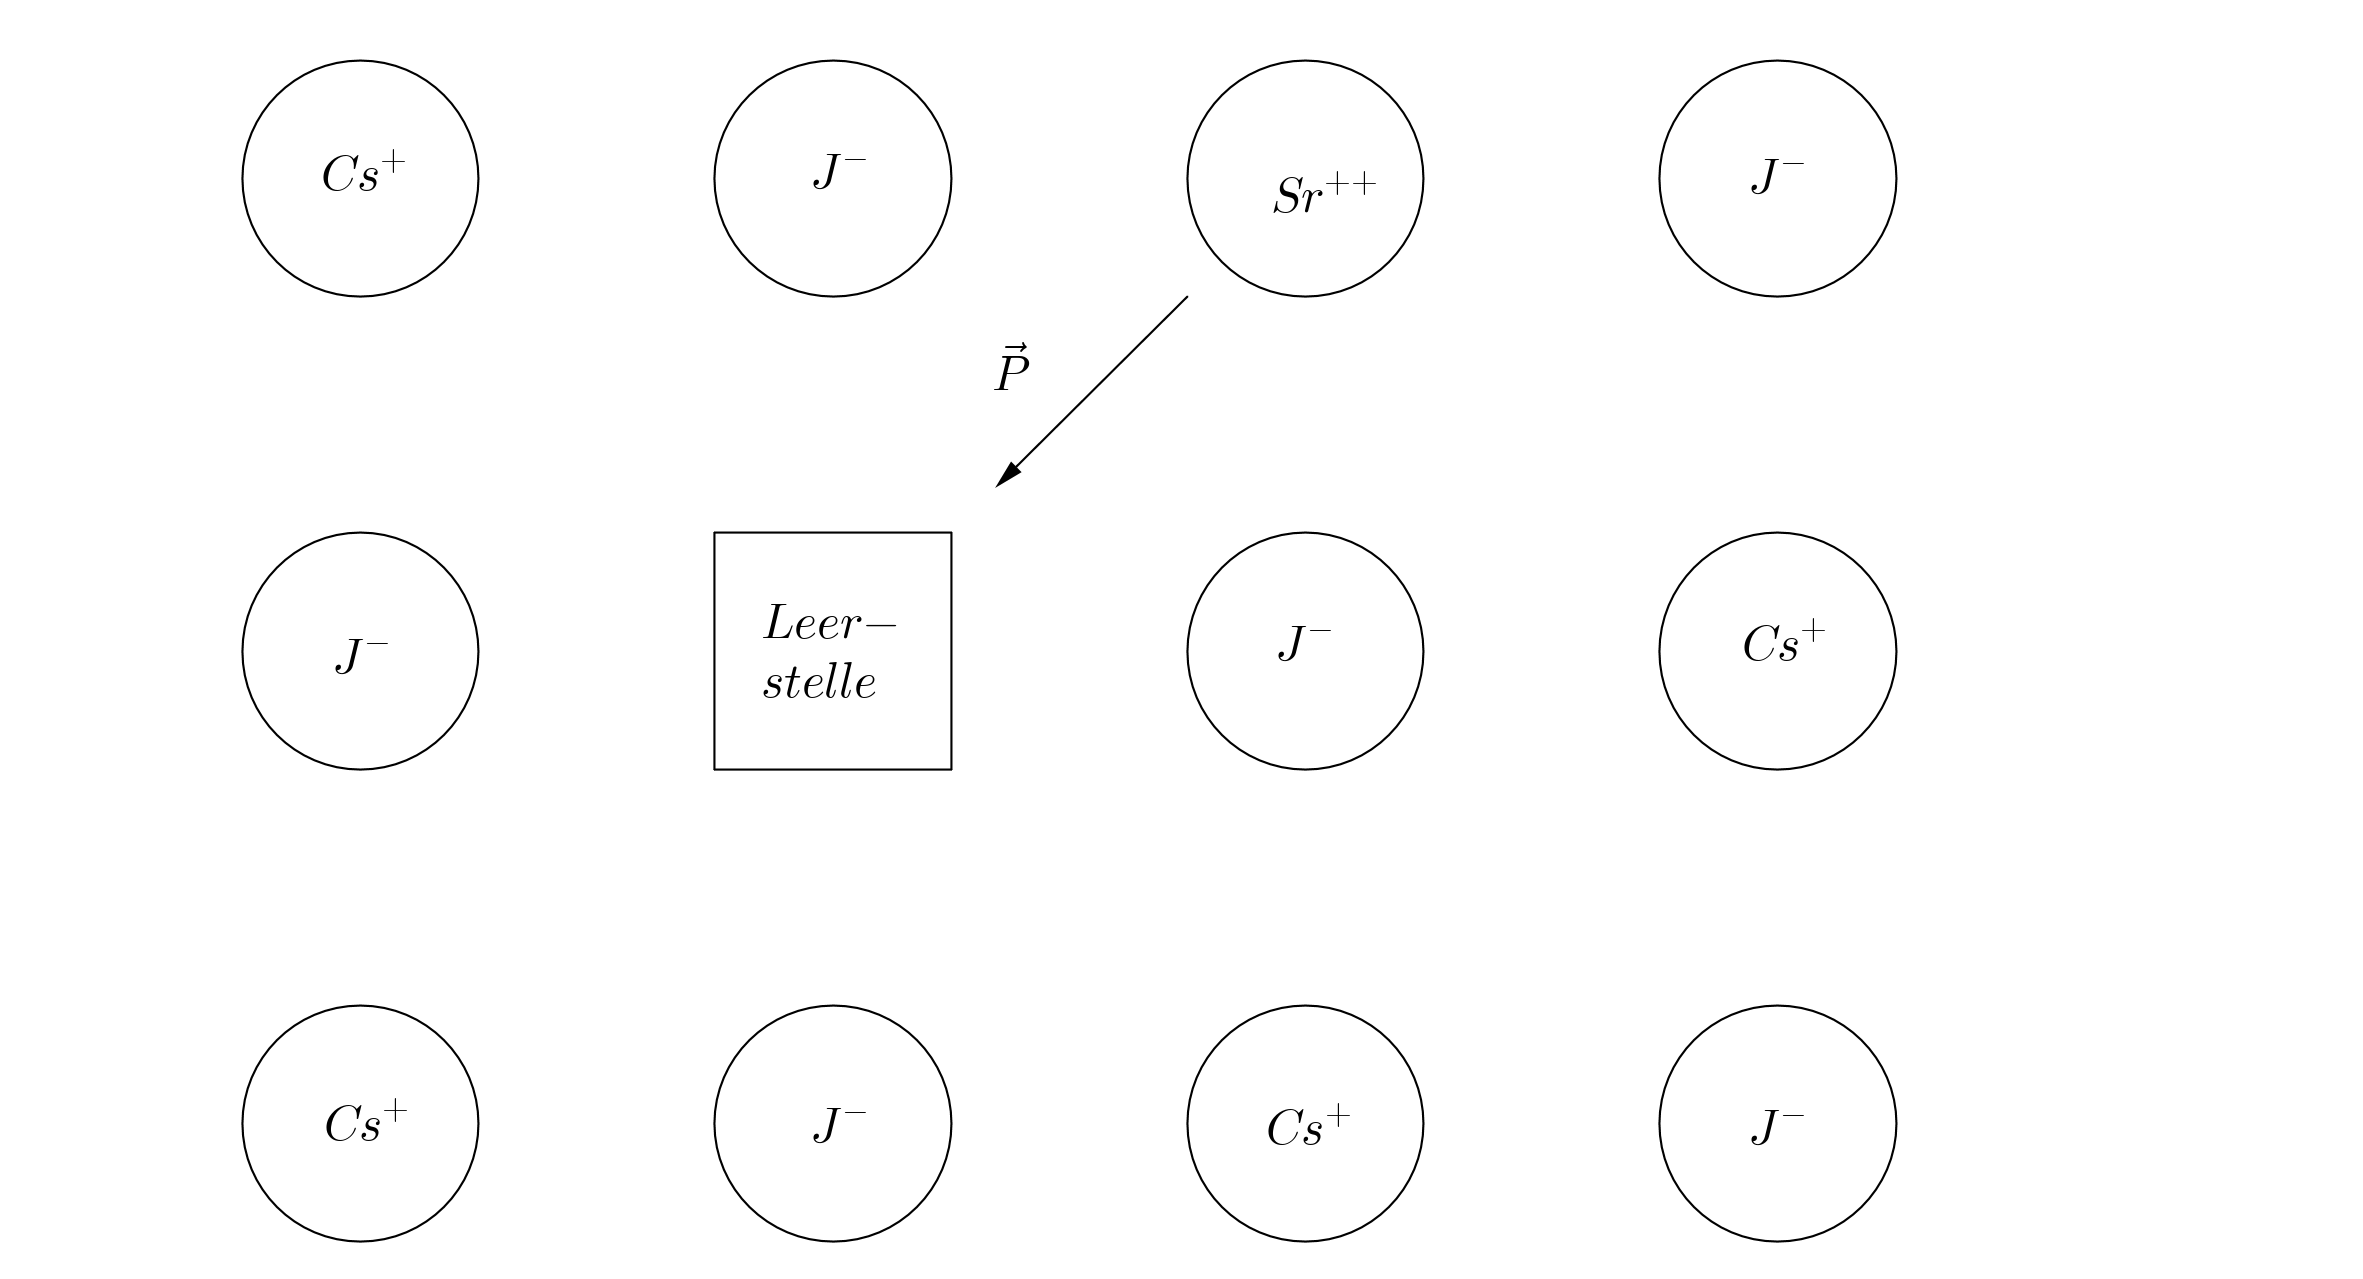
\includegraphics[width=\textwidth]{../pics/dipGitt.png}
\caption{Entstehung eines Dipols im Ionengitter}
\label{pic_dipGitt}
\end{figure}
Wegen der diskreten Gitterpunkte sind nur diskrete Dipolausrichtung möglich, wobei unterhalb von 500 $^\circ$C sich ausschließlich die Leerstellen bewegen.
Die Potentialschwelle die zu dieser Leerstellendiffusion die durch den periodischen Verlauf des Gitterpotentials festgelegt ist, muss überwunden werden.
Damit ist eine Aktivierungsenergie $W$ verbunden. Der Anteil der Dipole, die diese Energie mittels der thermischen Bewegung aufbringt ist
verteilt nach der Boltzmann-Statistik $\exp(W/k_B\,T)$, mit $k_B$ als Boltzmann-Konstante. Die mittlere Zeit einer Dipolumorientierung wird Relaxationszeit
$\tau$ genannt, die direkt proportional zur Boltzmann-Statistik sein muss
\begin{align}
 \tau(T) = \tau_0 \exp\left(\frac{W}{k_B\, T}\right),
 \label{eq_tau(W)}
\end{align}
mit $\tau_0$ als charakteristische Relaxationszeit, die bei unendlicher Temperatur bestehen würde. Im Versuch sollen die Aktivierungsenergie und die
charakteristische Relaxationszeit ermittelt werden.

\subsection{Messverfahren}
Die untersuchte mit Strontium dotierte Kaliumbromid-Probe ist kreisförmig und etwa 3-5 mm dick. Sie dient als Dielektrikum eines Plattenkondensators,
an den eine Gleichspannung angeschlossen wird, sodass innerhalb der Probe ein elektrisches Feld $E$ wirkt. Die statistisch ausgerichteten 
Dipole in der Probe richten sich entsprechend der Feldrichtung aus. Die Ausrichtung wird jedoch wird jedoch durch die thermische Bewegung der 
Gitterbausteine gestört, sodass nur ein Bruchteil $y$ der Dipole in Feldrichtung zeigt. Dieser Anteil wird durch die Langevin-Funktion $L(x)$
beschrieben
\begin{align}
 y = L(x) = \cot(x) - \frac{1}{x} \hspace{1cm}\text{mit }x=\frac{pE}{k_B T},
\end{align}
die für den Fall $pE\ll k_B T$ wird zu 
\begin{align}
 y = \frac{pE}{3k_B T}.
 \label{eq_y(T)}
\end{align}
Um tatsächlich diesen Bruchteil zu erhalten, muss das Feld lange gegenüber der Relaxationszeit eingeschaltet sein. Bei eingeschaltetem E-Feld wird
die Probe mit flüssigem Stickstoff schnell auf eine Temperatur $T_0$ gebracht. Wegen des exponentiellen Zusammenhangs, ist es möglich, diesen
Polarisationszustand konstant zu halten. Nach Abschalten des Felds, wird der Kondensator kurzgeschlossen, was den Ladungsteil bei tiefen Temperaturen
in Form von Elektronen verschwinden lässt. Mit konstanter Heizrate $b=\dx T/\dx t = const$ wird die Probe erhitzt, was dazu führt, dass die Dipole
sich wieder statistisch ausrichten werden. Dieser Vorgang wird Dipolrelaxation genannt und bringt einen Depolarisationsstrom mit sich, der mit einem
empfindlichen Strommessgerät gemessen werden kann. Zu Beginn steigt der Strom entsprechend Abbildung \ref{pic_i(T)} mit der Temperatur steil an, da $\tau$ schnell abnimmt, woraufhin er
ein Maximum erreicht und wieder abnimmt, da nicht relaxierte Dipole weniger werden. Die Depolarisationsstromdichte $j(T)$ setzt sich zusammen aus dem
Bruchteil $y$, der bei Polarisationstemperatur $T_p$ orientierten Dipole, dem Dipolmoment $p$ und der Zahl der pro Zeiteinheit relaxierenden Dipole
$\dx N/\dx t$
\begin{align}
 j(T) = y(T_p)\, p\, \frac{\dx N}{\dx t}.
 \label{eq_Depoldichte}
\end{align}
\begin{figure}[H]
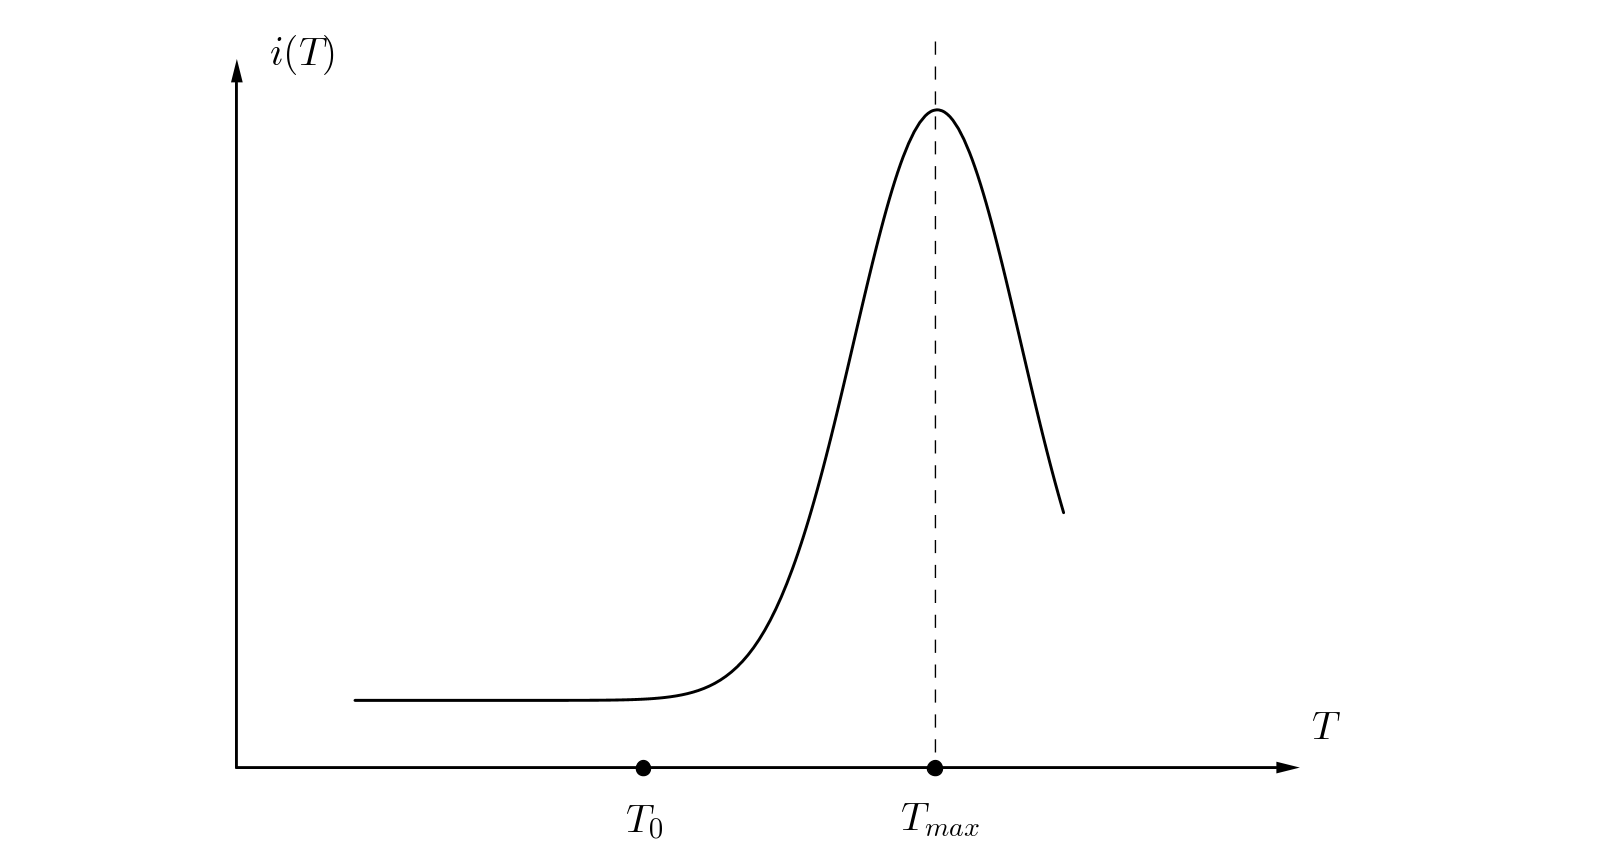
\includegraphics[width=\textwidth]{../pics/i(T).png}
\caption{Depolarisationsstromdichte}
\label{pic_i(T)}
\end{figure}
Nach \eqref{eq_y(T)} ergibt sich 
\begin{align}
 y(T_p)p=\frac{p^2E}{3k_BT_p},
\end{align}
da es sich bei der Dipolrelaxation um einen thermischen Prozess handelt, ist $\dx N/\dx t$ proportional zur noch vorhandenen Zahl orientierter Dipole,
wobei der Proportionalitätsfaktor die inverse Relaxationszeit ist
\begin{align}
 \frac{\dx N}{\dx t} = -\frac{N}{\tau(T)},
\end{align}
was eine Differentialgleichung darstellt, deren Lösung eine Exponentialfunktion darstellt und allsamt in \eqref{eq_Depoldichte} zu
\begin{align}
 j(T)=\frac{p^2E}{3k_BT_p}\frac{N_p}{\tau_0}\exp\left(-\frac{1}{b\tau_0}\int\limits_{T_0}^T \exp\left(\frac{W}{k_B\, T'}\right) \dx T'  \right) \exp\left(\frac{W}{k_B\, T}\right).
 \label{eq_jlang}
 \end{align}
Für das Anfangsintervall ist $\exp(W/k_BT)$ klein, was zur Näherung führt
\begin{align}
 j(T) \approx \frac{p^2E}{3k_BT_p}\frac{N_p}{\tau_0}\exp\left(\frac{W}{k_B\, T}\right)
 \label{eq_j(T)}
\end{align}
und in einem ($\ln j-1/T$)-Diagramm zu einer Geraden führt, aus deren Steigung sich die Aktivierungsenergie $W$ errechnen lässt. Größere Genauigkeit
hierbei liefert die Betrachtung des gesamten Kurvenverlaufs. Die Polarisation $P$ ist dem Gesamtdipolmoment pro Volumeneinheit entsprechend und
proportional zur Zahl orientierter Dipole. Beim Aufheizen gilt hier ebenfalls eine Relaxationsgleichung
\begin{align}
 \frac{\dx P}{\dx t} = - \frac{P(t)}{\tau(T(t))}.
\end{align}
Durch die Änderung der Polarisation wird ein äußerer Stromkreis $i$ erzeugt, der integriert führt zu
\begin{align}
 \int\limits_{t(T)}^\infty i(t)\dx t = \int\limits_{t(T)}^\infty F\frac{\dx P}{\dx t}\dx t = -FP(t),
\end{align}
wobei $P(\infty) = 0$. Durch einen linearen Zusammenhang von $t(T)$ und $T$ lässt sich nun schließlich $\tau$ schreiben als
\begin{align}
 \tau(T) = \frac{1}{b\,i(T)}\int\limits_T^\infty i(T')\dx T'
\end{align}
und mit \eqref{eq_tau(W)} die Aktivierungsenergie
\begin{align}
 W = k_BT \ln\left(\frac{1}{b\tau_0 i(T)}\int\limits_T^{T^*} i(T')\dx T'\right).
 \label{eq_int}
\end{align}
Durch Auftragen des $\ln$-Ausdrucks gegen $1/T$ kann $W$ aus dem Geradenanstieg errechnet werden, wobei $T^*$ eine beliebe, feste Temperatur ist,
bei der $i(T^*)\approx 0$. $\tau_0$ lässt sich nun indirekt aus der Lage von $T_{max}$ aus Abbildung \ref{pic_i(T)} bestimmen. Durch Differenziation
von \eqref{eq_jlang} ist eine Beziehung zwischen $T_{max}$ und $\tau(T_{max})$ herstellen. Durch Einsetzen des Wertepaars ($T_{max}$, $\tau(T_{max})$
in \eqref{eq_tau(W)} lässt sich schließlich die charakteristische Relaxationszeit $\tau_0$ bestimmen.

\section{Durchführung}
Im Versuch sollen für mit Strontium dotiertes Kaliumbromid $i-T$-Kurven bei zwei verschiedenen Heizraten $b$ zwischen $2^\circ$C/min und $8^\circ$C/min
aufgenommen werden. Der Temperaturverlauf der Relaxationszeit $\tau(T)$ soll angegeben werden, sowie die Aktivierungsenergie $W$ durch beide vorgestellten
Methoden berechnet werden.
\begin{figure}[H]
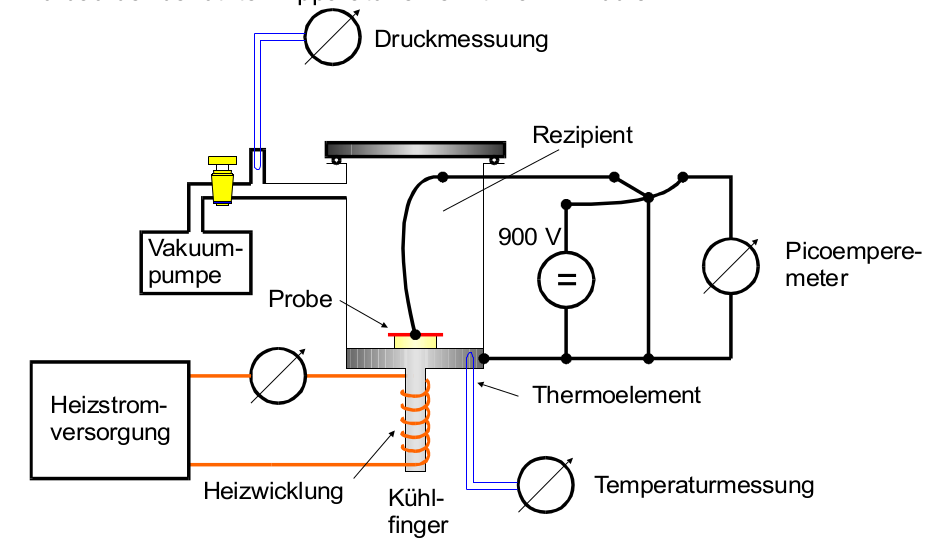
\includegraphics[width=\textwidth]{../pics/dipolAufbau.png}
\caption{Schematischer Aufbau der Messapparatur}
\label{pic_dipolaufbau}
\end{figure}
Die Probe befindet sich auf dem Boden des Probenbehälters. Da die Kristalle hygroskopisch sind, muss der Probenbehälter auf etwa 10$^{-2}$ bar
evakuiert werden. Anschließend wird das elektrische Feld bei einer Spannung zwischen $U = 600-900$ V über 900 s bei $T_p=320$ K erzeugt. Nach der
Polarisation wird die Probe mit flüssigem Stickstoff auf 210 K gekühlt. Das E-Feld wird abgeschaltet und der Kondensator entladen. Nun wird das
Picoamperemeter angeschlossen und bei stabiler Anzeige der Aufheizprozess begonnen. Um konstante Heizraten zu erhalten ist es nötig den Temperaturverlauf
ständig beobachten und die Heizleistung nach Tabelle \ref{tab_heizrate} angepasst werden.
\begin{table}[H]
 \begin{tabular}{c|c|c}
 $b$ in $^\circ$C/min & $T$ in $^\circ$C & $I_{Heiz}$ in A\\
 \hline
 \multirow{8}{0mm}{2} &-50&0,8\\
 &-18 & 0,9\\
 &-3 & 1,0 \\
 &+5 & 1,1 \\
 &+33 & 1,2 \\
 &+44 & 1,3 \\
 &+52 & 1,4 \\
 &+58 & 1,5 \\
 \hline
 \multirow{6}{0mm}{3} &-50&1,0\\
 &-20&1,1\\
 &+2&1,3\\
 &+28&1,4\\
 &+41&1,5\\
 &+51&1,7\\
 \hline
 \multirow{6}{0mm}{4} &-50&1,5\\
 &-30&1,6\\
 &-7&1,7\\
 &+25&2,0\\
 &+44&2,2\\
 &+65&2,5\\
 \hline
 \multirow{6}{0mm}{5} &-50&1,7\\
 &-16&2,0\\
 &+26&2,2\\
 &+44&2,3\\
 &+60&2,6\\ 
 \end{tabular}
\caption{Heizstrom für konsante Temperaturerhöhungen bei verschiedenen Heizraten}
\label{tab_heizrate}
\end{table}

\section{Auswertung}
Bei diesem Versuch wird die durch ein Amperemeter gemessene Stromstäker in Abhängigkeit von der Probentemperatur aufgezeichnet. Aufgenommen wurden folgende zwei Messreihen\\
\begin{table}
\begin{minipage}{0.45\textwidth}
\begin{tabular}{c|c}
Temp. [$C^\circ$] & Strom [$10^{-12}A$]\\\hline
-61,1	&0,05\\\hline
-59,1	&0,01\\\hline
-55,6	&0,04\\\hline
-53,5	&0,50\\\hline
-52,2	&0,70\\\hline
-50,6	&2,50\\\hline
-48,5	&3,00\\\hline
-46,6	&3,30\\\hline
-44,7	&3,50\\\hline
-42,9	&3,50\\\hline
-41,1	&3,50\\\hline
-39,5	&4,00\\\hline
-37,8	&3,50\\\hline
-36,2	&4,00\\\hline
-34,4	&3,90\\\hline
-32,7	&4,20\\\hline
-30,9	&4,00\\\hline
-29,1	&4,20\\\hline
-27,2	&4,10\\\hline
-25,2	&4,10\\\hline
-23,1	&4,20\\\hline
-21,0	&4,30\\\hline
-18,9	&4,20\\\hline
-16,9	&4,00\\\hline
-14,7	&4,10\\\hline
-13,0	&4,00\\\hline
-11,2	&3,90\\\hline
-5,3	&4,10\\\hline
-7,6	&3,50\\\hline
\end{tabular}
\end{minipage}
\begin{minipage}{0.45\textwidth}
\begin{tabular}{c|c}
Fortsetzung & \\\hline
-5,8	&3,50\\\hline
-4,1	&3,40\\\hline
-2,2	&3,20\\\hline
-0,1	&3,00\\\hline
2,2		&2,80\\\hline
4,5		&2,20\\\hline
6,6		&2,30\\\hline
8,3		&2,00\\\hline
10,0	&1,80\\\hline
11,8	&1,30\\\hline
14,0	&1,20\\\hline
16,3	&0,50\\\hline
18,7	&0,00\\\hline
20,8	&0,00\\\hline
22,9	&0,01\\\hline
24,9	&0,12\\\hline
26,9	&0,14\\\hline
28,8	&0,15\\\hline
30,6	&0,20\\\hline
32,5	&0,25\\\hline
34,5	&0,33\\\hline
36,6	&0,41\\\hline
38,7	&0,50\\\hline
40,8	&0,62\\\hline
42,8	&0,75\\\hline
44,7	&0,92\\\hline
48,6	&4,50\\\hline
50,4	&4,00\\\hline
\end{tabular}
\end{minipage}
\caption{Messwerte der ersten Messreihe}
\label{tab_werte1}
\end{table}

\begin{table}
\begin{minipage}{0.45\textwidth}
\begin{tabular}{c|c}
Temp. [$C^\circ$] & Strom [$10^{-12}A$]\\\hline
-58,9	&3,00\\\hline
-56,0	&4,90\\\hline
-49,3	&5,20\\\hline
-41,3	&5,60\\\hline
-35,1	&6,00\\\hline
-30,3	&6,10\\\hline
-26,2	&6,10\\\hline
-22,1	&6,10\\\hline
-17,7	&6,10\\\hline
-12,9	&6,30\\\hline
-7,9	&6,20\\\hline
-2,9	&6,20\\\hline
2,0		&6,10\\\hline
6,9		&6,00\\\hline
11,9	&6,00\\\hline
16,7	&5,80\\\hline
\end{tabular}
\end{minipage}
\begin{minipage}{0.45\textwidth}
\begin{tabular}{c|c}
Fortsetzung & \\\hline
21,7	&5,70\\\hline
26,7	&5,60\\\hline
31,7	&5,40\\\hline
36,7	&5,30\\\hline
41,5	&5,20\\\hline
46,3	&5,00\\\hline
51,6	&4,80\\\hline
57,0	&4,20\\\hline
62,1	&3,70\\\hline
66,9	&2,70\\\hline
71,4	&1,30\\\hline
76,0	&0,60\\\hline
80,8	&0,60\\\hline
85,9	&0,65\\\hline
90,8	&1,00\\\hline
\end{tabular}
\end{minipage}
\caption{Messwerte der zweiten Messreihe}
\label{tab_werte2}
\end{table}

Trägt man beide Messreihen in ein Diagramm ein, so wird ersichtlich, das der Nullpunkt linear mit der Temperatur angehoben wird. Um dieses Verhalten heraus zu korrigieren, wird mit einer Regressionsgeraden die Steigung bestimmt und die Kurve um diesen Wert abgesenkt. In Diagramm \ref{pic_dia1} und \ref{pic_dia1} sind sowohl Messwerte als auch die lineare Regression eingezeichnet.

\begin{figure}[htbp]
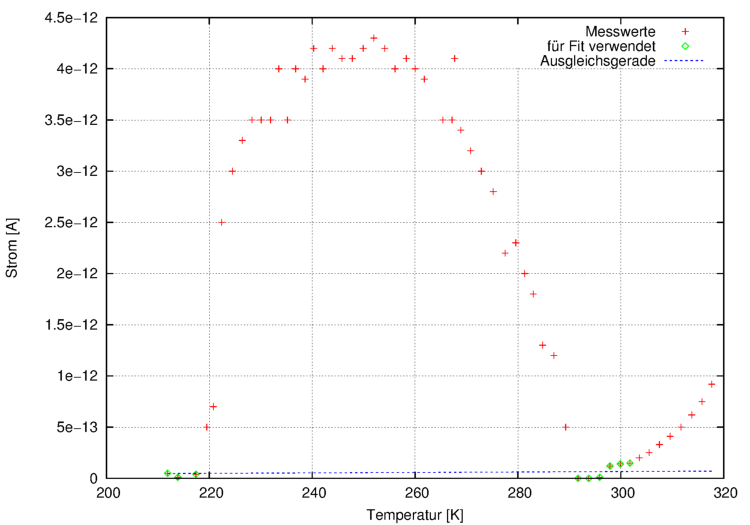
\includegraphics[scale=0.8]{../gnu/relax11.pdf}
\caption{Erste Messreihe. Die in grün umrahmten Werte wurden für die lineare Regression mit einer Geraden durch den Ursprung benutzt.}
\label{pic_dia1}
\end{figure}
\begin{figure}[htbp]
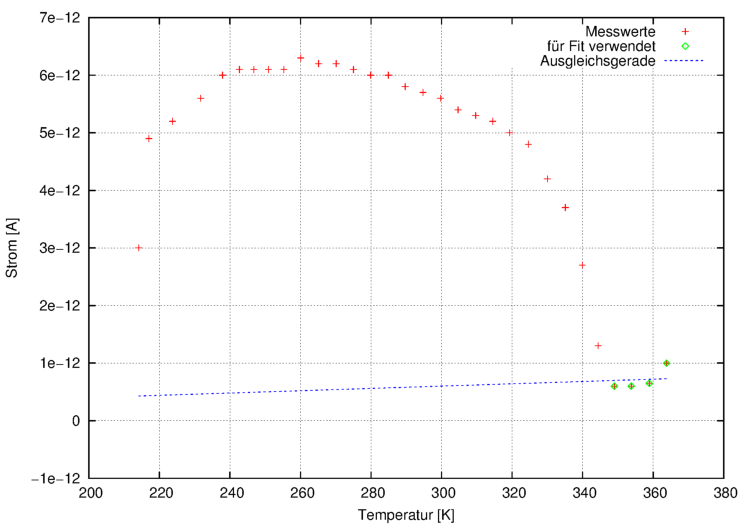
\includegraphics[scale=0.8]{../gnu/relax12.pdf}
\caption{Zweite Messreihe. Die in grün umrahmten Werte wurden für die lineare Regression mit einer Geraden durch den Ursprung benutzt.}
\label{pic_dia2}
\end{figure}

Als Fitparameter wurde die Steigung $m_i$ der beiden Geraden verwendet. Folgende Werte wurden errechnet:\\
\begin{align}
m_1&=(2,21     \pm 0,73) \cdot10^{-16} \frac{A}{T}\\
\label{eq_korr1}
m_2&=( 2,00  \pm0,26)\cdot10^{-15}\frac{A}{T}
\end{align}

\subsection{Erste Methode}
Im Folgenden wurden die in \eqref{eq_korr1} berechneten Korrekturen bereits angewendet. Es soll nun die Aktivierungsenergie $W$ berechnet werden. Dazu wird ausgenutzt, dass für den frühen Kurvenverlauf die Gesetzmäßigkeit in \eqref{eq_j(T)} gilt. Aus den korrigierten Werte wird daher der Logarithmus gebildet und dieser dann gegen $\frac{1}{x}$ aufgetragen. Die Kurven sind in Abbildung \ref{pic_21} und \ref{pic_22} Die Steigung der Geraden entspricht der Aktivierungsenergie.\\

\begin{figure}[H]
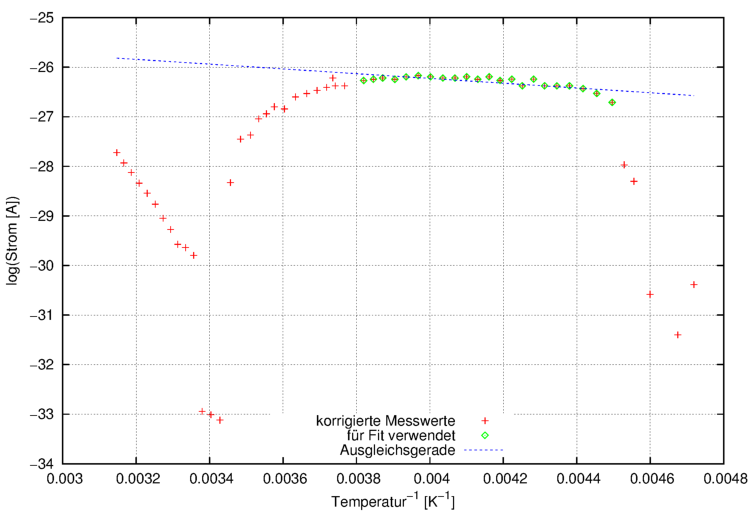
\includegraphics[scale=0.8]{../gnu/relax21.pdf}
\caption{Erste Messreihe logarithmisch aufgetragen. Die in grün umrahmten Werte wurden für die lineare Regression verwendet}
\label{pic_21}
\end{figure}

Es wurden folgende Aktivierungsenergien gemessen:
\begin{align}
W_1&=(-3,48\pm 0,67)\cdot10^{25} J\\
W_2&=(-2,298 \pm 0,29)\cdot10^{25} J
\end{align}
\begin{figure}[H]
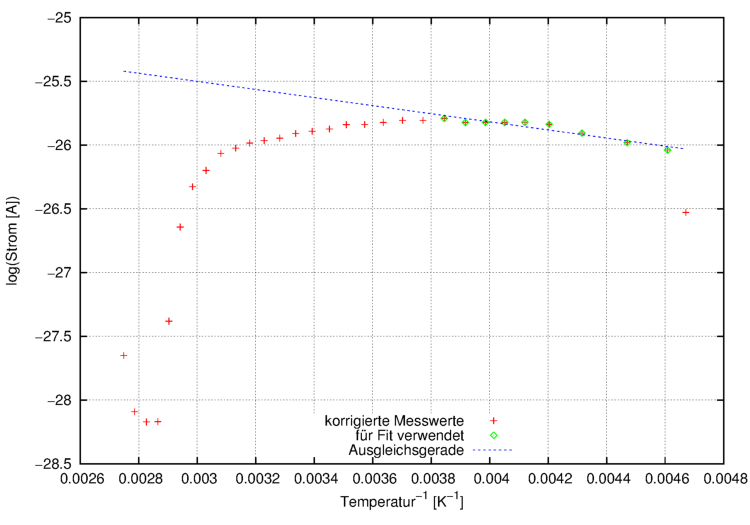
\includegraphics[scale=0.8]{../gnu/relax22.pdf}
\caption{Zweite Messreihe logarithmisch aufgetragen. Die in grün umrahmten Werte wurden für die lineare Regression verwendet}
\label{pic_22}
\end{figure}

\subsection{Zweite Methode}
Anschließend wird die Aktivierungsenergie über eine zweite Methode bestimmt. Entsprechend Gleichung \eqref{eq_int} lässt sich die Aktivierungsenergie auch durch die Fläche der Kurve bestimmen. Aus den Messpunkte wird dafür mittels der Trapezregel die Kurvenfläche bestimmt und diese dann gegen $\frac{1}{T}$ aufgetragen. Die durch Integration erhaltenen Werte stehen in Tabellen \ref{tab_int1} und \ref{tab_int2}. Es ergibt sich dabei der Graph in Abbildungen \ref{pic_int1} und \ref{pic_int2}. Die Aktivierungsenergie lässt sich wieder als Steigung der Ausgleichsgeraden ablesen.

\begin{table}[htbp]
\begin{minipage}[t]{0.45\textwidth}
\centering
\begin{tabular}{c|c}
Temperatur $[C^\circ]$ & $\int ^{T^*}_{T} i(T')dT'$\\\hline
-59,1 &245,11\\\hline
-55,6 &245,02\\\hline
-53,5 &244,46\\\hline
-52,2 &243,68\\\hline
-50,6 &241,12\\\hline
-48,5 &235,34\\\hline
-46,6 &229,36\\\hline
-44,7 &222,90\\\hline
-42,9 &216,60\\\hline
-41,1 &210,30\\\hline
-39,5 &204,30\\\hline
-37,8 &197,92\\\hline
-36,2 &191,92\\\hline
-34,4 &184,81\\\hline
-32,7 &177,93\\\hline
-30,9 &170,55\\\hline
-29,1 &163,17\\\hline
-27,2 &155,28\\\hline
-25,2 &147,08\\\hline
-23,1 &138,37\\\hline
-21,0 &129,44\\
\end{tabular}
\end{minipage}
\begin{minipage}[t]{0.45\textwidth}
\centering
\begin{tabular}{c|c}
Fortsetzung & \\\hline
-18,9 &120,52\\\hline
-16,9 &112,32\\\hline
-14,7 &103,41\\\hline
-13,0 &96,52\\\hline
-11,2 &89,41\\\hline
-9,3 &65,81\\\hline
-7,6 &57,07\\\hline
-5,8 &50,77\\\hline
-4,1 &44,91\\\hline
-2,2 &38,64\\\hline
-0,1 &32,13\\\hline
2,2 &25,46\\\hline
4,5 &19,71\\\hline
6,6 &14,98\\\hline
8,3 &11,33\\\hline
10,0 &8,10\\\hline
11,8 &5,31\\\hline
14,0 &2,56\\\hline
16,3 &0,60\\\hline
18,7 &0,00\\\hline
\end{tabular}
\end{minipage}
\caption{Messwerte, die durch Integration der zweiten Messreihe entstanden sind. Verwendet wurde die Trapez-Methode }
\label{tab_int1}
\end{table}

\begin{table}[htbp]
\begin{minipage}[t]{0.45\textwidth}
\centering
\begin{tabular}{c|c}
Temperatur $[C^\circ]$ & $\int ^{T^*}_{T} i(T')dT'$\\\hline
-58,9 &700,535\\\hline
-56,0 &689,08\\\hline
-49,3 &655,245\\\hline
-41,3 &612,045\\\hline
-35,1 &576,085\\\hline
-30,3 &547,045\\\hline
-26,2 &522,035\\\hline
-22,1 &497,025\\\hline
-17,7 &470,185\\\hline
-12,9 &440,425\\\hline
-7,9 &409,175\\\hline
-2,9 &378,175\\\hline
2,0 &348,04\\\hline
6,9 &318,395\\
\end{tabular}
\end{minipage}
\begin{minipage}[t]{0.45\textwidth}
\centering
\begin{tabular}{c|c}
Fortsetzung & \\\hline
11,9 &288,395\\\hline
16,7 &260,075\\\hline
21,7 &231,325\\\hline
26,7 &203,075\\\hline
31,7 &175,575\\\hline
36,7 &148,825\\\hline
41,5 &123,625\\\hline
46,3 &99,145\\\hline
51,6 &73,175\\\hline
57,0 &48,875\\\hline
62,1 &28,73\\\hline
66,9 &13,37\\\hline
71,4 &4,37\\\hline
76,0 &0,0\\\hline
\end{tabular}
\end{minipage}
\caption{Messwerte, die durch Integration der ersten Messreihe entstanden sind. Verwendet wurde die Trapez-Methode}
\label{tab_int2}
\end{table}

\begin{figure}[H]
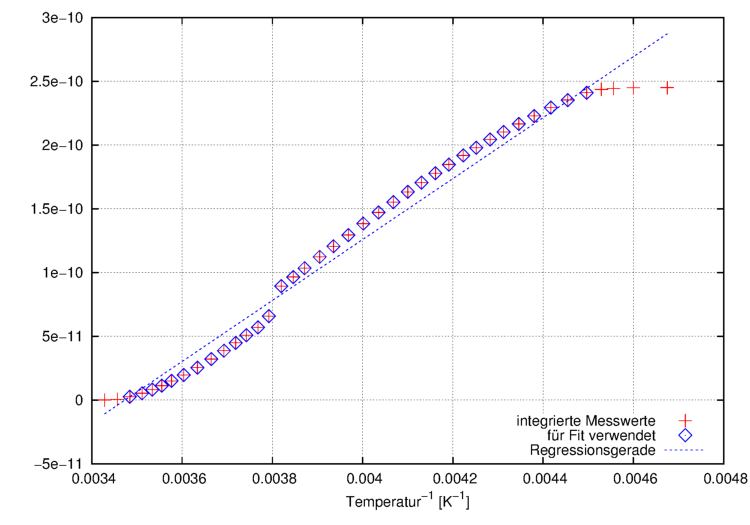
\includegraphics[scale=0.8]{../gnu/relax31.pdf}
\caption{Integrierte Werte der ersten Messreihe gegen $\frac{1}{T}$ aufgetragen. Die blau umrahmten Werte wurden für die lineare Regression verwendet}
\label{pic_int1}
\end{figure}
\begin{figure}[H]
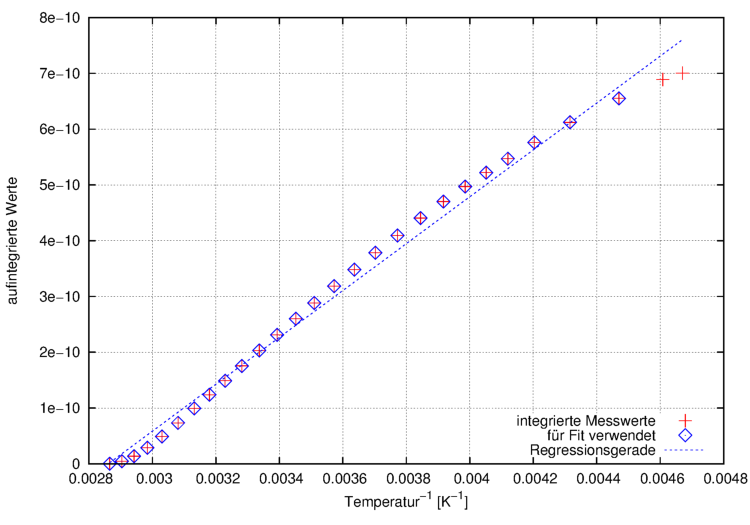
\includegraphics[scale=0.8]{../gnu/relax32.pdf}
\caption{Integrierte Werte der zweiten Messreihe gegen $\frac{1}{T}$ aufgetragen. Die blau umrahmten Werte wurden für die lineare Regression verwendet}
\label{pic_int2}
\end{figure}

Es wurden folgende Aktivierungsenergien gemessen:
\begin{align}
W_1&=(1,73    \pm 0,041)\cdot 10^{16} J\\
W_2&=(3,04	\pm 0,06)\cdot 10^{16}J
\end{align}

\section{Diskussion und Fazit}
Die Berechnung der Aktivierungsenergie gelang mit beiden Methoden ohne große statistische Abweichungen. Dennoch liegen die Werte um 9 Größenordnungen auseinander. Plausibler sind die Werte, die mit der zweiten Methode bestimmt wurden. Diese liegen im Bereich von 1keV.\\
Gut sichtbar wird bei den integrierten Werten in Abbildung \ref{pic_int1} ein Sprung der Messwerte, der jedoch das Ergebnis hier nicht weiter beeinflusst, da nur die Steigung der Ausgleichsgeraden von Bedeutung ist. Es ist jedoch gut möglich, dass sich dieser Sprung bei Verwendung der ersten Methode stärker bemerkbar macht und somit die Diskrepanz der Ergebnisse teilweise erklärt. Der Sprung rührt vermutlich daher, dass zu diesem Zeitpunkt die Sensibilität des Amperemeters verändert wurde.\\


\parskip 340pt
\Large{Literatur}\\\\

% ========================================
%	Literaturverzeichnis
% ========================================

%\bibliographystyle{plainnat}			% Bibliographie-Style auswählen
%\bibliography{BIBDATEI}			% Literaturverzeichnis

% ========================================
%	Das Dokument endent
% ========================================

\end{document}
